\documentclass{article}

\usepackage[utf8]{inputenc}
\usepackage[hidelinks]{hyperref}
\usepackage{graphicx}

\renewcommand{\thesection}{}
\renewcommand{\thesubsection}{}

\graphicspath{{img/}}

\title{
	ocp-lint-web\\
    User Manual
}
\date{}
\author{}

\begin{document}

\maketitle

\newpage

\tableofcontents

\newpage

\section{Introduction}
\vspace{\baselineskip}

\paragraph{}
\texttt{ocp-lint} is static OCaml code analyzer make for detect uses of patterns known to ease the hidden presence of bugs. Initially, the results were printed on the standard output but \texttt{ocp-lint} can raise hundreds of warnings on a project and it is often hard for a developer to deal with them.

\paragraph{}
\texttt{ocp-lint-web} is a GUI for \texttt{ocp-lint} usable on any web browser.
It permit a fluent navigation through the errors and the warnings raised on your project.
The tool is fully written in OCaml with Js\_of\_ocaml compiler and his syntax extension.

\paragraph{}
First, the web output must be generated by the option \textit{--output-web} of \texttt{ocp-lint} that will make the index and the others required static pages (especially the files contents).
Then, you can navigate through the \texttt{ocp-lint} warnings.

\newpage

\section{Home page}
\vspace{\baselineskip}

\paragraph{}
\frame{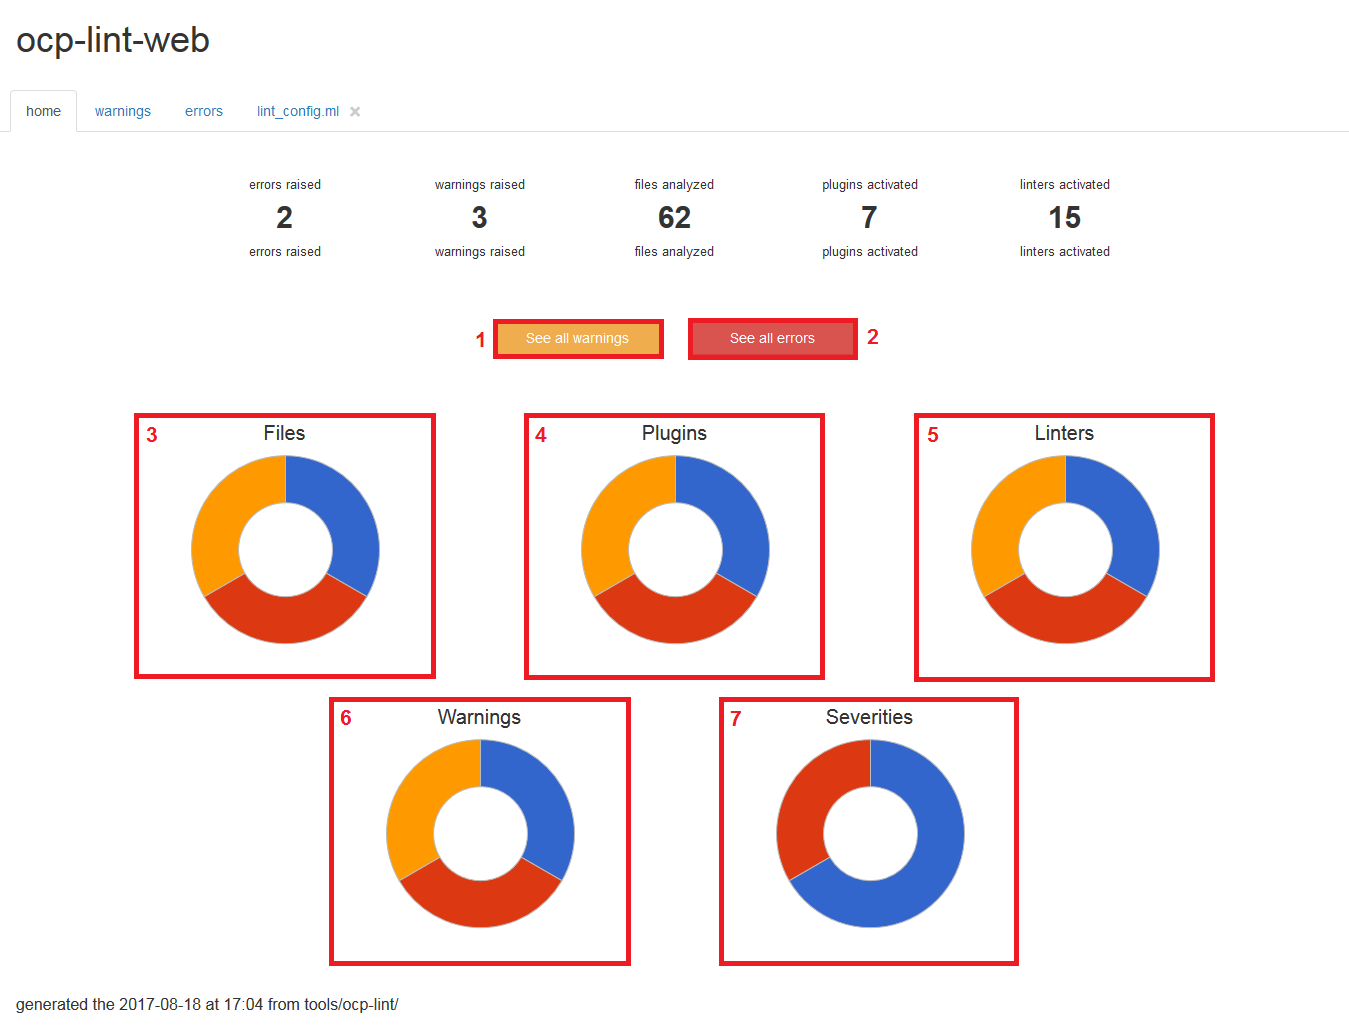
\includegraphics[width=\textwidth,keepaspectratio=true]{ocp_lint_web_home.png}}

\vspace{\baselineskip}

\paragraph{}
This is the first page you see when you launch \texttt{ocp-lint-web}. It contains some informations on you project analysis such as the number of activated plugins or the pie of the warnings returned group by file.

\paragraph{}
\begin{itemize}
	\item[1 -] Warnings button : Permit to open the Warnings page.
	\item[2 -] Errors button : Permit to open the Errors page.
    \item[3 -] File pie : Show the number of raised warnings group by file. Clicking in a part of the pie (except the part \textit{other}) will open the File page of the specified file.
    \item[4 -] Plugin pie : Show the number of raised warnings group by plugin.
    \item[5 -] Linter pie : Show the number of raised warnings group by linter.
    \item[6 -] Warning pie : Show the number of raised warnings group by warning.
    \item[7 -] Severity pie : Show the number of raised warnings group by severity.
\end{itemize}

\newpage

\section{Warnings page}
\vspace{\baselineskip}

\paragraph{}
\frame{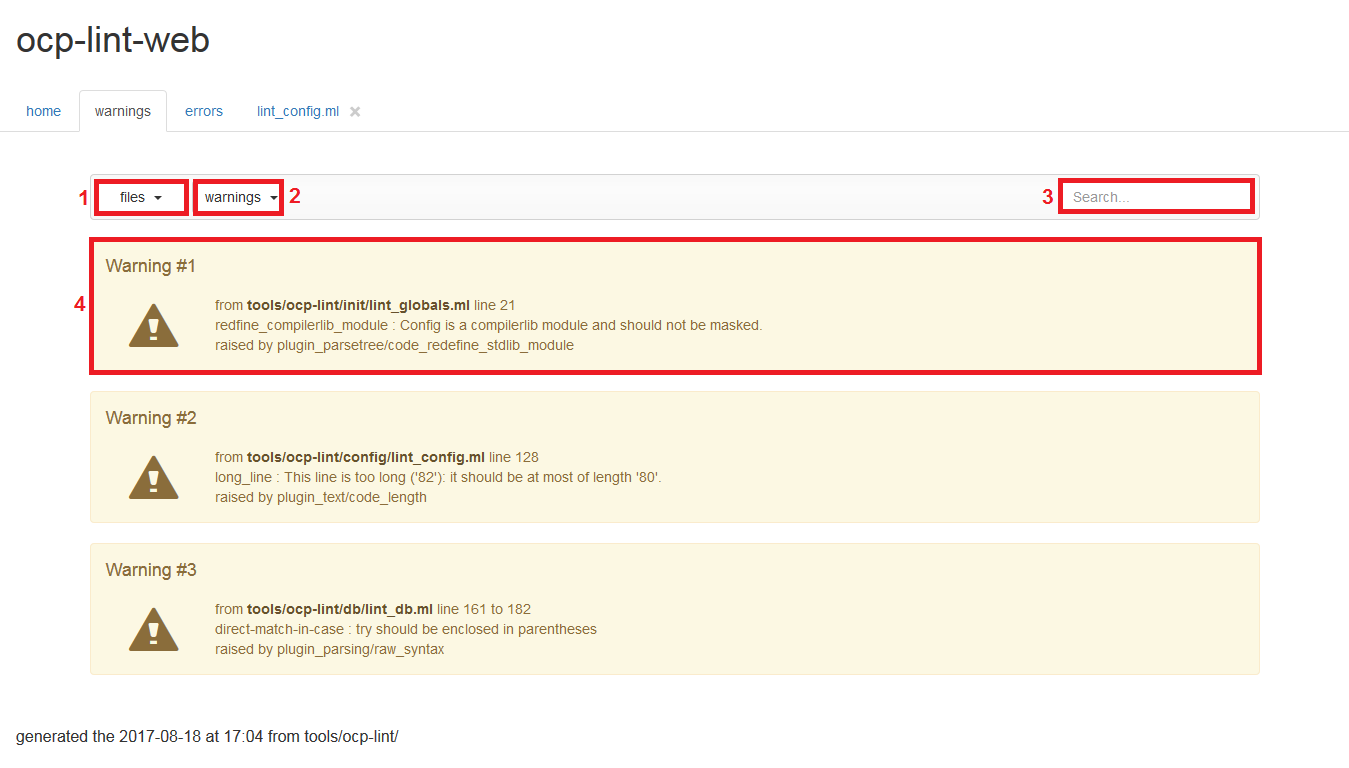
\includegraphics[width=\textwidth,keepaspectratio=true]{ocp_lint_web_warnings.png}}

\vspace{\baselineskip}

\paragraph{}
This page present all the warnings emit by \texttt{ocp-lint} on your project.

\paragraph{}
\begin{itemize}
	\item[1 -] File filter : Permit to display only the warnings from the checked files of the dropdown menu.
	\item[2 -] Warning filter : Permit to display only the checked warnings of the dropdown menu.
    \item[3 -] Searchbox : Permit to display only the warnings that contains the keyword in the text input.
    \item[4 -] Warning summary : Show a short description of the warning. Clicking on it will open the File page of the specified warning.
\end{itemize}

\newpage

\section{Errors page}
\vspace{\baselineskip}

\paragraph{}
\frame{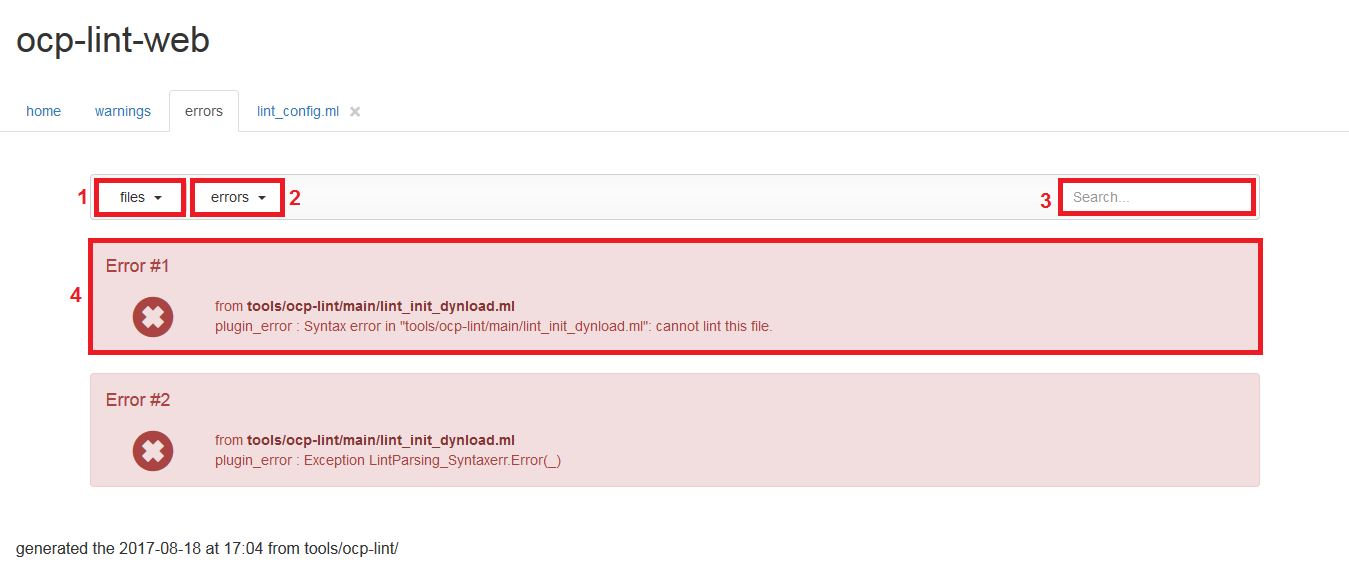
\includegraphics[width=\textwidth,keepaspectratio=true]{ocp_lint_web_errors.png}}

\vspace{\baselineskip}

\paragraph{}
This page present all the errors emit by \texttt{ocp-lint} on your project.

\paragraph{}
\begin{itemize}
	\item[1 -] File filter : Permit to display only the errors from the checked files of the dropdown menu.
	\item[2 -] Error filter : Permit to display only the checked errors of the dropdown menu.
    \item[3 -] Searchbox : Permit to display only the errors that contains the keyword in the text input.
    \item[4 -] error summary : Show a short description of the error. Clicking on it will open the File page of the specified error.
\end{itemize}

\newpage

\section{File page}
\vspace{\baselineskip}

\paragraph{}
\frame{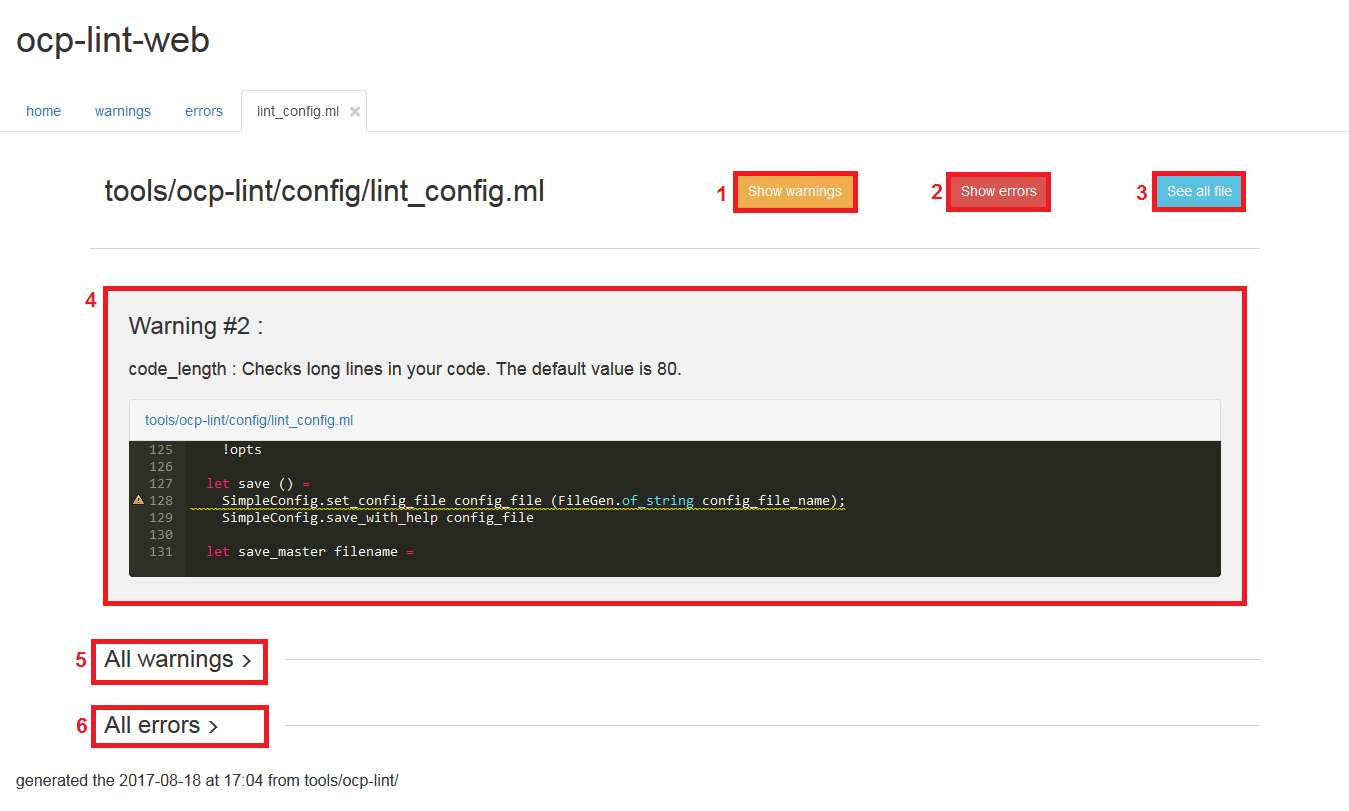
\includegraphics[width=\textwidth,keepaspectratio=true]{ocp_lint_web_file.png}}

\vspace{\baselineskip}

\paragraph{}
This page is a summary of the errors and warnings throws by the specified file. You can navigate through the warnings and see their attached part of code.

\paragraph{}
\begin{itemize}
	\item[1 -] Warnings button : Permit to unfold the list of the raised warnings content of the file.
	\item[2 -] Errors button : Permit to unfold the list of the raised errors content of the file.
    \item[3 -] File : Permit to see all the file in the main panel.
    \item[4 -] Main panel : Show the current select content all. It can contains a warnings, an error or all the file.
    \item[5 -] Warnings tittle : Permit to fold/unfold the warnings content of the file.
    \item[6 -] Errors tittle : Permit to fold/unfold the list of the errors content of the file.
\end{itemize}

\newpage


\subsection{Warnings content}
\vspace{\baselineskip}

\paragraph{}
\frame{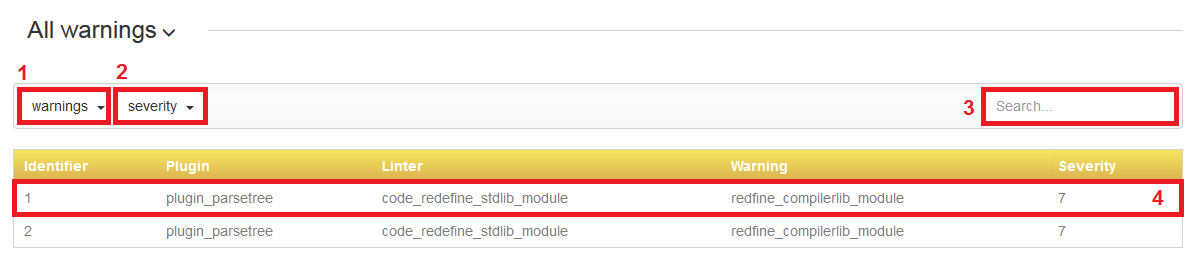
\includegraphics[width=\textwidth,keepaspectratio=true]{ocp_lint_web_file_warnings.png}}

\vspace{\baselineskip}

\paragraph{}
This menu permit to show in details the warnings of the selected file.

\paragraph{}
\begin{itemize}
	\item[1 -] Warning filter : Permit to display only the checked warnings of the dropdown menu in the table.
    \item[2 -] Severity filter : Permit to display only the warnings with an higher severity than selected of the dropdown menu in the table.
    \item[3 -] Searchbox : Permit to display only the warnings that contains the keyword in the text input.
    \item[4 -] Warning entry : Show some details of the warning. Clicking on it will open this warning in the main panel.
\end{itemize}

\newpage


\subsection{Errors content}
\vspace{\baselineskip}

\paragraph{}
\frame{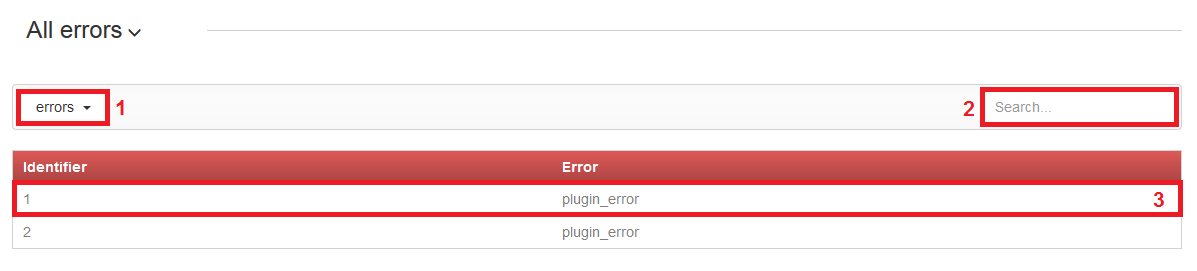
\includegraphics[width=\textwidth,keepaspectratio=true]{ocp_lint_web_file_errors.png}}

\vspace{\baselineskip}

\paragraph{}
This menu permit to show in details the errors of the selected file.

\paragraph{}
\begin{itemize}
	\item[1 -] Error filter : Permit to display only the checked errors of the dropdown menu in the table.
    \item[2 -] Searchbox : Permit to display only the errors that contains the keyword in the text input.
    \item[3 -] Error entry : Show some details of the error. Clicking on it will open this error in the main panel.
\end{itemize}
    
\end{document}
